\begin{exercises} 


\item Let $E(x,y) = \ds \frac{100}{1+(x-5)^2 + 4(y-2.5)^2}$ represent the elevation on a land mass at location $(x,y)$.  Suppose that $E$, $x$, and $y$ are all measured in meters.
    \ba
    \item Find $E_x(x,y)$ and $E_y(x,y)$.

    \item Let $\vu$ be a unit vector in the direction of $\langle -4,3 \rangle$.  Determine $D_{\vu} E(3,4)$.  What is the practical meaning of $D_{\vu} E(3,4)$ and what are its units?

    \item Find the direction of greatest increase in $E$ at the point $(3,4)$.

    \item Find the instantaneous rate of change of $E$ in the direction of greatest decrease at the point $(3,4)$.  Include units on your answer.
    
    \item At the point $(3,4)$, find a direction $\vw$ in which the instantaneous rate of change of $E$ is 0.

    \ea

\begin{exerciseSolution}
\ba 
\item For this function $E$ we have 
\[E_x(x,y) = -\frac{200(x-5)}{(1+(x-5)^2 + 4(y-2.5)^2)^2} \ \ \text{ and } \ \ E_y(x,y) = -\frac{800(y-2.5)}{(1+(x-5)^2 + 4(y-2.5)^2)^2}.\]

\item A unit vector in the direction of $\langle -4,3 \rangle$ is $\vu = \frac{1}{5} \langle -4, 3 \rangle$. Since
\[E_x(3,4) = \frac{100}{49} \ \ \text{ and } \ \ E_y(3,4) = -\frac{300}{49},\]
we have
\[D_{\vu} E(3,4) = \nabla E(3,4) \cdot \vu = \left\langle \frac{100}{49}, -\frac{300}{49} \right\rangle \cdot \frac{1}{5} \langle -4,3 \rangle = \frac{20}{49} (-4 - 9) = -\frac{260}{49} \approx -5.306 \ \frac{\text{meters}}{\text{meter}}.\]
For every one meter change in the direction of $\vu$ from the point $(3,4)$, the elevation decreases by $\frac{260}{49}$ meters. 
 
\item The direction of greatest increase of $E$ at the point $(3,4)$ is 
\[\nabla E (3,4) = \langle E_x(3,4), E_y(3,4) \rangle = \frac{100}{49} \langle 1, -3 \rangle \approx \langle 2.04, -6.12 \rangle.\]

\item The direction of greatest decrease of $E$ at $(3,4)$ is $-\nabla E(3,4)$. The instantaneous rate of change of $E$ in the direction of greatest decrease at the point $(3,4)$ is
\[-|\nabla E(3,4)| = -\frac{100}{49}\sqrt{1+9} = -\frac{100}{49}\sqrt{10} \approx -6.454 \ \frac{\text{meters}}{\text{meter}}.\]

\item We want a direction vector $\vw = \langle w_1, w_2 \rangle$ so that 
\[0 = D_{\vw} E(3,4) = \nabla E(3,4) \cdot \vw = \left\langle \frac{100}{49}, -\frac{300}{49} \right\rangle \cdot \langle w_1, w_2 \rangle = \frac{100}{49}(w_1-3w_2).\]
So the vector $\langle 3, 1 \rangle$ is a direction in which $E$ does not change at the point $(3,4)$.
\ea


\end{exerciseSolution}

\item Let $f(x,y) = x^2+3y^2$.
    \ba
    \item Find $\nabla f(x,y)$ and $\nabla f(1,2)$.

    \item Find the direction of greatest increase in $f$ at the point $(1,2)$. Explain. A graph of the surface defined by $f$ is shown in Figure \ref{F:10.6.Grad_ex}. Illustrate this direction on the surface.

    \item A contour diagram of $f$ is shown in Figure \ref{F:10.6.Grad_ex_contours}. Illustrate your calculation from (b) on this contour diagram.
\begin{figure}[ht]
\begin{center}
\begin{minipage}{2.5in}
\begin{center}
%\resizebox{!}{2.4in}{\includegraphics{10_6_Grad_ex_surface}}
  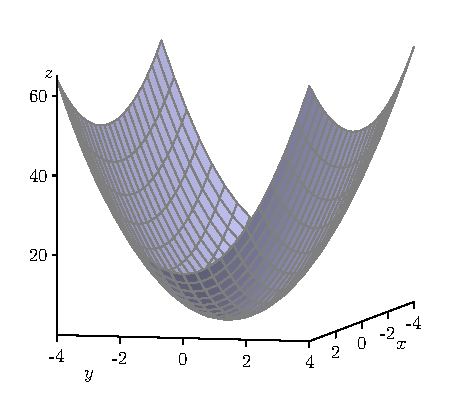
\includegraphics{figures/fig_10_6_exercise_graph.eps}
\end{center}
\caption{The surface for $f(x,y) = x^2+3y^2$.}
\label{F:10.6.Grad_ex}
\end{minipage} \hspace{0.5in}
\begin{minipage}{2.5in}
\begin{center}
%\resizebox{!}{2.2in}{\includegraphics{10_6_Grad_ex_contours}}
  \includegraphics{figures/fig_10_6_exercise_contour.eps}
\end{center}
\caption{Contours for $f(x,y) = x^2+3y^2$.}
\label{F:10.6.Grad_ex_contours}
\end{minipage}
\end{center}
\end{figure}

	\item Find a direction $\vw$ for which the slope of the tangent line to the surface generated by $f$ at the point $(1,2)$ is zero in the direction $\vw$.

    \ea

\begin{exerciseSolution}
\ba 
   \item In this case we have
\[\nabla f = \langle f_x, f_y \rangle = \langle 2x, 6y \rangle.\]
 Evaluating $\nabla f$ at $(1,2)$ gives us
\[\nabla f(1,2) = \langle 2, 12 \rangle.\]

	\item The gradient shows the direction of greatest increase of $f$ at a point. An illustration of this direction at the point $(1,2,f(1,2))$ is shown in the figure below, with the gradient vector scaled appropriately to make it easier to plot. 
\begin{center}
\resizebox{!}{2.2in}{\includegraphics{figures/fig_10_6_Ex_surface_gradient}}
\end{center}

	\item The gradient shows the direction of greatest increase of $f$ at a point. The gradient is perpendicular to the level curves, and a picture of the unit vector in the direction of the gradient at $(1,2)$ is shown in the figure below, with the gradient vector scaled appropriately to make it easier to plot.  
\begin{center}
\resizebox{!}{2.2in}{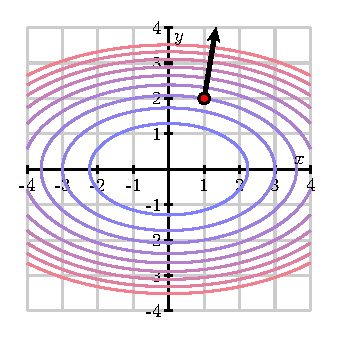
\includegraphics{figures/fig_10_6_Ex_contour_gradient}}
\end{center}

	\item We need to find a direction $\vw = \langle w_1, w_2 \rangle$ so that $D_{\vw} f(1,2) = \nabla f(1,2) \cdot \vw = 0$. Since $\nabla f (1,2)= \langle 2, 6 \rangle$, we need $w_1$ and $w_2$ to satisfy $2w_1+6w_2=0$. So $w_1=-3w_2$ and a direction for which the slope of the tangent line to the surface generated by $f$ at the point $(1,2)$ is zero in the direction $\vw$ is $\langle -3,1 \rangle$. 

\ea

\end{exerciseSolution}


\item The properties of the gradient that we have observed for functions of two variables also hold for functions of more variables.  In this problem, we consider a situation where there are three independent variables.  Suppose that the temperature in a region of space is described by
  $$
  T(x,y,z) = 100e^{-x^2-y^2-z^2}
  $$
  and that you are standing at the point $(1,2,-1)$.
  \ba
\item Find the instantaneous rate of change of the temperature in the direction of
  $\vv=\langle 0, 1, 2\rangle$ at the point $(1,2,-1)$.  Remember that you should first find a
  {\em unit} vector in the direction of $\vv$.

\item In what direction from the point $(1,2,-1)$ would you move to cause the temperature to
  decrease as quickly as possible?

\item How fast does the temperature decrease in this direction?

\item Find a direction in which the temperature does
  not change at $(1,2,-1)$.

  \ea


\begin{exerciseSolution}
  \ba
\item A unit vector in the direction of $\vv$ is $\vu = \frac{1}{\sqrt{5}} \vv$. The instantaneous rate of change of the temperature in the direction of
  $\vv=\langle 0, 1, 2\rangle$ is then
\begin{align*}
\left| \nabla T(1,2,-1) \cdot \vu \right| &= \left| \langle T_x(1,2,-1), T_y(1,2,-1), T_z(1,2,-1) \rangle \cdot \vu \right| \\
	&= \left| \left\langle -200e^{-6}, -400e^{-6}, 200e^{-6} \right\rangle \cdot \frac{1}{\sqrt{5}} \langle 0,1,2\rangle \right| \\
	&= \left|-80\sqrt{5}\left\langle 0, e^{-6}, -e^{-6} \right\rangle \right| \\
	&= 80\sqrt{5}\sqrt{2}e^{-6} \\
	&\approx 0.627. \\
\end{align*}

\item To cause the temperature to decrease as quickly as possible we move in the direction of 
\[-\nabla T(1,2,-1) = \left\langle 200e^{-6}, 400e^{-6}, -200e^{-6} \right\rangle \approx \langle 0.5, 1, -0.5 \rangle.\]


\item The rate of change of the temperature in this direction is 
\[\left|\nabla T(1,2,-1) \right| =  200 \sqrt{6}e^{-6} \approx 1.21.\]
So the temperature decreases at approximately 1.21 in this direction.

\item Let $\vu = \langle u_1, u_2, u_3 \rangle$ be a vector in a direction in which the temperature does not change. Then
\begin{align*}
0 &= \nabla T(1,2,-1) \cdot \vu \\
	&= \left\langle -200e^{-6}, -400e^{-6}, 200e^{-6} \right\rangle \cdot \langle u_1, u_2, u_3 \rangle \\
	&= -200e^{-6}(u_1+2u_2-u_3).
\end{align*}
So a direction in which the temperature does not change is the direction of the vector $\langle -1,1,1 \rangle$. 


  \ea
\end{exerciseSolution}

\item Figure \ref{F:10.6.gradient.field} shows a plot of the gradient
  $\nabla f$ at several points for some function $f(x,y)$.

  \begin{figure}[ht]
    \begin{center}
     \includegraphics{figures/fig_10_6_gradient_field.eps}
    \end{center}	
    \caption{The gradient $\nabla f$.}
    \label{F:10.6.gradient.field}
  \end{figure}

  \ba
\item Consider each of the three indicated points, and draw, as best
  as you can, the contour through that point.

\item Beginning at each point, draw a curve on which $f$ is continually
  decreasing. 

  \ea

\begin{exerciseSolution}
  \ba
\item Since the gradient at a point is orthogonal to the contour at that point, the contours through the indicated points are drawn orthogonal to the gradients. This is illustrated in the figures below.

\begin{center}
\resizebox{!}{1.5in}{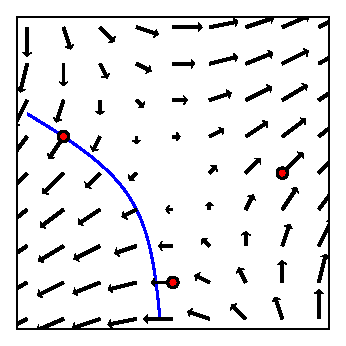
\includegraphics{figures/fig_10_6_Ex_4_a_1}} \hspace{0.1in} \resizebox{!}{1.5in}{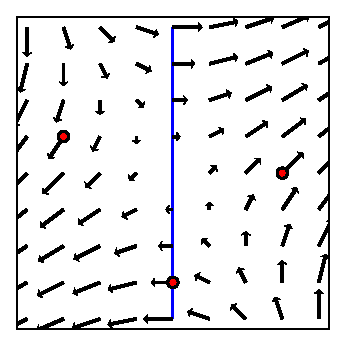
\includegraphics{figures/fig_10_6_Ex_4_b_1}}  \hspace{0.1in} \resizebox{!}{1.5in}{\includegraphics{figures/fig_10_6_Ex_4_c_1}}
\end{center}


\item The gradient points in the direction of the greatest increase of the function, so a curve that moves in the direction opposite the gradient is a curve on which $f$ is decreasing. This is illustrated in the figures below.

\begin{center}
\resizebox{!}{1.5in}{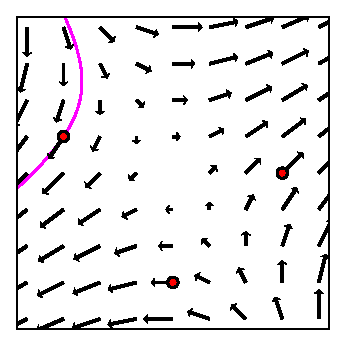
\includegraphics{figures/fig_10_6_Ex_4_a_2}} \hspace{0.1in} \resizebox{!}{1.5in}{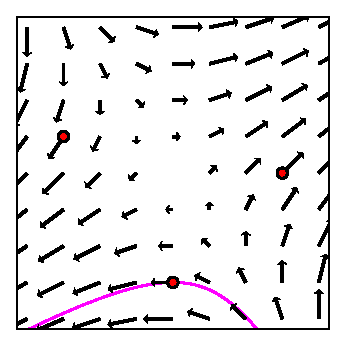
\includegraphics{figures/fig_10_6_Ex_4_b_2}}  \hspace{0.1in} \resizebox{!}{1.5in}{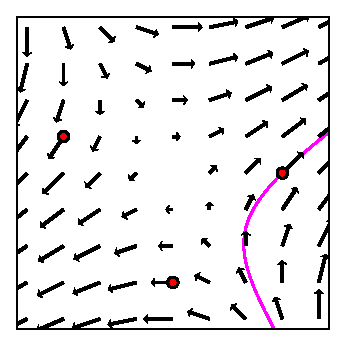
\includegraphics{figures/fig_10_6_Ex_4_c_2}}
\end{center}
  \ea
\end{exerciseSolution}

\end{exercises}

\afterexercises
